\chapter{Úvod}\label{chap:uvod}
\addcontentsline{toc}{chapter}{Úvod}

Spolu s harmonií a rytmem představuje melodie základní stavební kámen většiny existující hudby. V průběhu vývoje od folklórních zpěvů přes orchestrální skladby po soudobou elektroniku si melodie téměř vždy zachovávala své dominantní postavení nositele esence jednotlivých písní. Melodie je to hlavní, co si člověk po poslechu skladby odnáší a nejsnadněji vybaví, a její důležitost je zejména v našem kulturním kontextu natolik jednoznačná, že je občas těžké si bez ní vůbec hudbu představit. 

Tato práce se zabývá metodami odhadu fundamentální frekvence melodie ze zvukové nahrávky. Jinými slovy chceme získat v každém bodě vstupní skladby informaci o tom, zda melodie zní a její případnou výšku. Jde o jednu z nejdůležitějších a zároveň nejtěžších úloh z oboru \textit{Music Information Retrieval}, jejíž rozsah využití v této doméně pokrývá významnou část aktivně řešených, otevřených problémů. Spolehlivý přepis melodie by usnadnil vyhledávání v hudebních datech, ať už na základě notového zápisu (\textit{Symbolic Melodic Similarity}), pomocí nekvalitní nahrávky z rádia (\textit{Audio Fingerprinting}), pomocí broukání (\textit{Query by Singing/Humming}) nebo dokonce pomocí coveru hledané písně (\textit{Audio Cover Song Identification}). Mimo vyhledávání by byl algoritmus užitečný pro další zpracování zvukového signálu, ať už pro manipulaci a úpravu melodického hlasu (například software Melodyne), nebo naopak jeho odstranění a vytvoření karaoke doprovodu (\textit{Informed Source Separation}). V neposlední řadě by extrakce melodie pomohla při kategorizaci hudebních dat, například podle žánru (\textit{Genre Classification}, \cite{Salamon2012}) nebo podle zpěváka (\textit{Singer Characterization}). A konečně široké spektrum využití by nalezla i v muzikologii (případně etnomuzikologii) pro kvantitativní i kvalitativní studii hudebních motivů a postupů (V jazzu například \cite{Pfleiderer}).

\begin{figure}[h]\centering
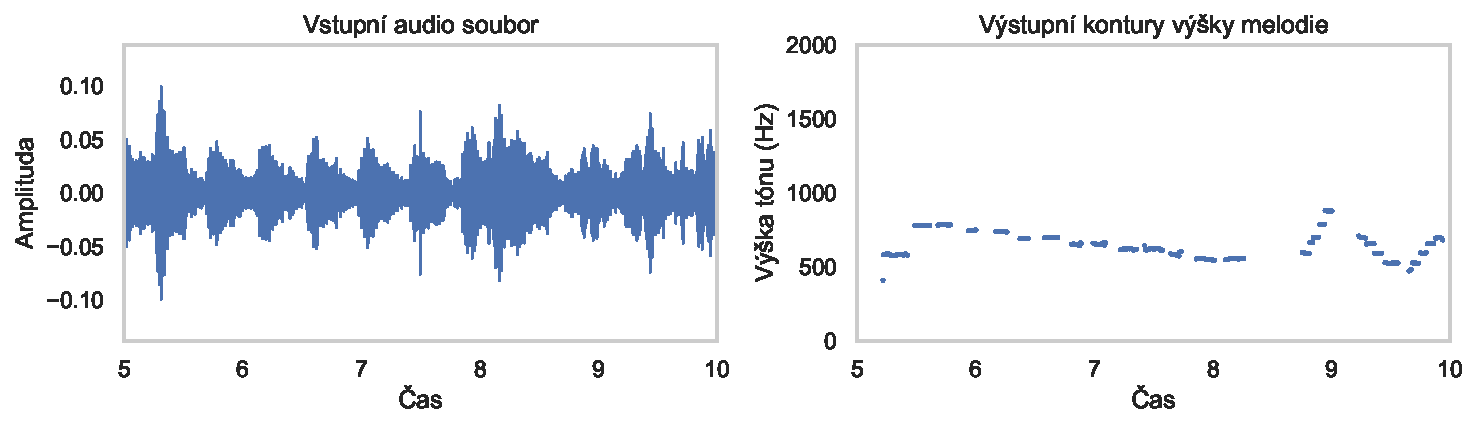
\includegraphics[width=\textwidth,height=\textheight,keepaspectratio]{../img/input_output}
\caption{Příklad vstupu a výstupu metody pro extrakci melodie. \textcolor{red}{přidat zvukový přílkad do přílohy}}
\label{obr:input_output}
\end{figure}

Extrakce melodie však nemusí sloužit pouze jako mezikrok pro řešení jiné úlohy, užitečný je i samotný výstup algoritmu, znázorněný na obrázku \ref{obr:input_output}. Motivačním příkladem použití může být pomoc při transkripci. Představíme-li si začínajícího hráče na saxofon, který si chce do not přepsat své oblíbené jazzové sólo, výstup algoritmu mu dá užitečnou informaci o tom, jaký tón zní v jakou chvíli. Z této reprezentace už pak hráči zbývá nalezené tóny projít a zapsat je do notové osnovy.

Proč je ale extrakce melodie otevřený problém? Příbuzná úloha, která spočívá v přepisu nahrávky jednoho izolovaného nástroje, je v podstatě vyřešena \citep{Mauch2014a}, proč se tato úloha po přidání hudebního doprovodu stává výrazně obtížnější? Pro vysvětlení dvou zásadních obtíží, které se s přepisem nahrávky pojí, musíme nejdříve přiblížit vůbec povahu zvuku a možnosti jeho zkoumání.


Naše zkušenost se zvukem probíhá primárně skrze sluch. Teprve na hlasitém koncertu však člověk pocítí, že zvuk je ve své fyzikální podstatě změna tlaku vzduchu, putující od zdroje k posluchači. Díky sluchu z těchto vibrací dokážeme oddělit jednotlivé zdroje a identifikovat v nich i velmi jemné rozdíly. Ačkoli jde o subjektivní vjemy, zvuky lze částečně rozřadit podle toho, jak snadno v nich rozeznáme nějakou konkrétní výšku. 

\vspace*{0.5cm}

Čtenář této práce si nyní může postupně vybavit: hrající violoncello, odbíjení kostelního zvonu, cinknutí příboru, štěkot psa, plynutí potoka, šelest listí stromů, trhání papíru, tlesknutí a prasknutí balónku.

\vspace*{0.5cm}

Se ztrácející se zřetelností výšky nejprve přijdeme o možnost zpívat společně se zdrojem zvuku v harmonii a posléze i o možnost si představit \uv{vyšší} a \uv{nižší} instance toho samého zvuku (jak zní vysoké a nízké prasknutí balónku?). To, co mají první z uvedených příkladů společné, je výrazná a stabilní periodicita jejich signálu --- daný tlakový průběh se opakuje v čase. Díky sluchu tuto periodicitu interpretujeme jako výšku, přičemž různé výšky se od sebe liší frekvencí, se kterou se signál opakuje. Hudební nástroje jsou jedním ze zdrojů těchto pravidelných vibrací, jejichž frekvenci lze zpravidla měnit (pomocí klapek, pohybu prstu po struně, atd.). Hlas nástroje však není charakteristický pouze svou výškou, nýbrž i barvou. Ta je určena podobou signálu v rámci jedné periody. 

\begin{figure}[h]\centering
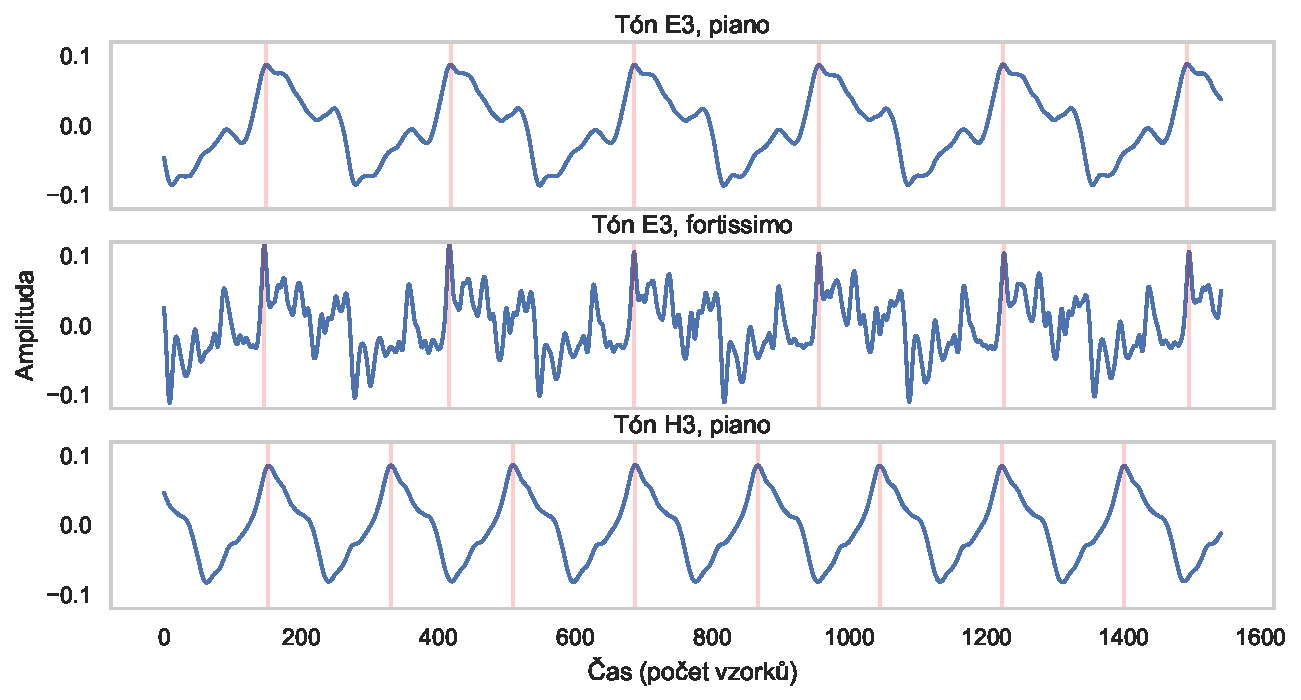
\includegraphics[width=\textwidth,height=\textheight,keepaspectratio]{../img/audio_clarinet}
\caption{Zvuk klarinetu, tóny s různou výškou a dynamikou, 25 milisekund signálu se vzorkovací frekvencí $44\,100\,\rm Hz$. \textcolor{red}{nějak uvést zdroj zvuku \url{https://www.philharmonia.co.uk/explore/sound_samples/clarinet?p=3}}}
\label{obr:audio_clarinet}
\end{figure}

Na obrázku \ref{obr:audio_clarinet} můžeme srovnat tři tóny hrané klarinetem, první dva mají stejnou výšku, jsou ale zahrané s různou intenzitou (dynamikou) \textcolor{red}{je tohle správně formulované, vím že dynamika není intenzita, ale \uv{zahrané s různou dynamikou} mi zní divně?}. Jejich vizuální rozdíl částečně odpovídá i rozdílu v barvě tónu, první tón má příjemný, měkký zvuk; druhý je výraznější a hrubší. Třetí tón se od zbylých liší svou výškou, což lze pozorovat na kratší periodě signálu, která je na obrázku vyznačená úsečkami. 

\begin{figure}[h]\centering
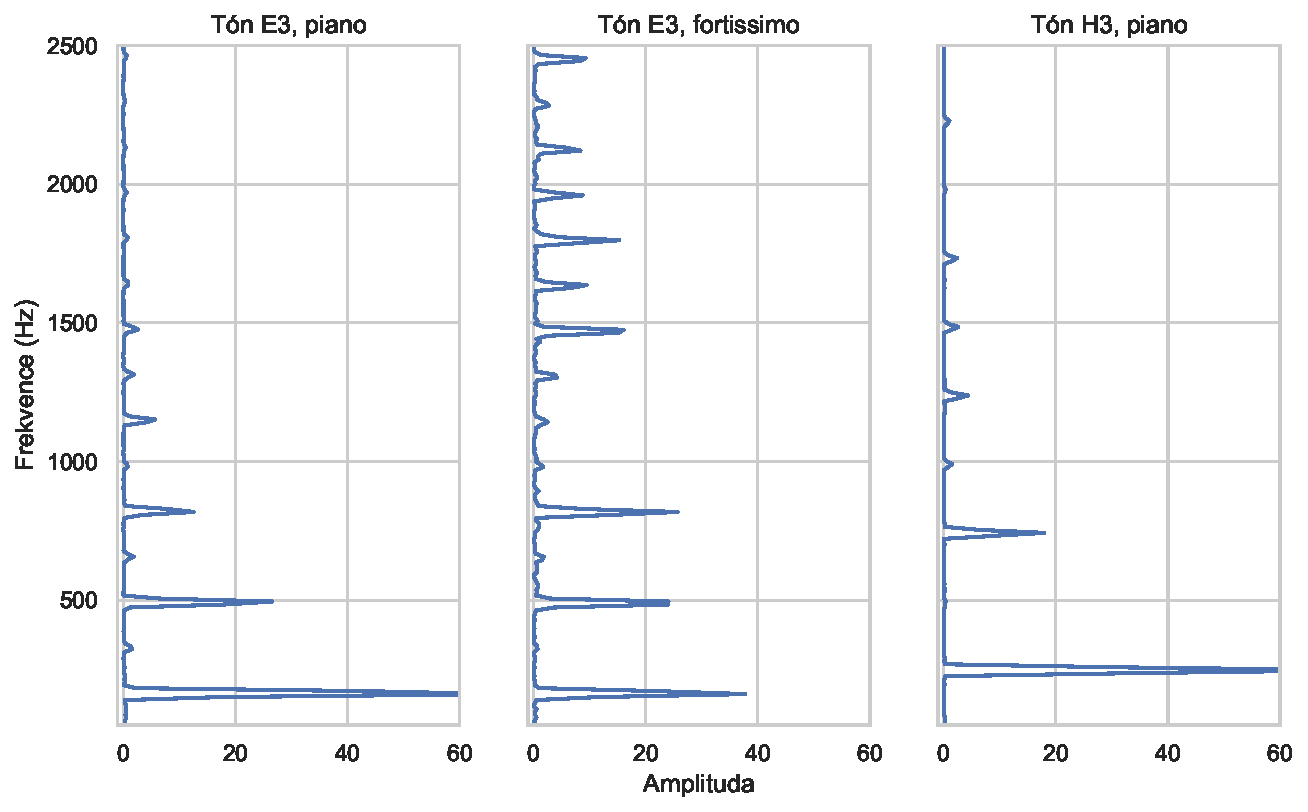
\includegraphics[width=\textwidth,height=\textheight,keepaspectratio]{../img/audio_clarinet_dft}
\caption{Zvuk klarinetu, absolutní hodnota výstupu Fourierovy tranformace signálu délky 4096 s oknem typu Hamming.}
\label{obr:audio_clarinet_dft}
\end{figure}

Jedním ze způsobů analýzy zvukového signálu je pomocí Fourierovy transformace (DFT). Základní myšlenkou je, že na signál lze hledět jako na vážený součet jednodušších signálů. Podobně, jako když se barvy na obrazovce míchají ze tří základních, libovolný zvuk můžeme smíchat ze sady sinusoid. Na obrázku \ref{obr:audio_clarinet_dft} vidíme část výsledku Fourierovy transformace zvuků klarinetu z předchozího příkladu. To zásadní, co na spektru tónu můžeme pozorovat, je jeho podstata jakožto součet \emph{harmonických složek}. Tón, kterému posluchač přisoudí výšku $f_0$, se zpravidla skládá ze součtu sinusoid, jejichž frekvence je celočíselným násobkem základní frekvence $f_0$. Například tedy tón E3 se na obrázku \ref{obr:audio_clarinet_dft} skládá z frekvencí $165\,\rm Hz$, $330\,\rm Hz$, $495\,\rm Hz$, \dots, zároveň intenzita těchto harmonických frekvencí určuje barvu hlasu.

Ukazuje se, že práce s touto reprezentací zvuku je pro analýzu signálu užitečnější, než práce s nezpracovaným signálem. Ze spektrální reprezentace je například na první pohled zřejmý vztah frekvencí porovnávaných signálů, který odpovídá lidské intuici o výšce zvuků --- tón E3 je na obrázku \ref{obr:audio_clarinet_dft} opravdu \uv{výš} než tón H3. Jak si také můžeme všimnout na spektru, pro hlas klarinetu platí, že liché harmonické frekvence jsou mnohem výraznější než sudé (například druhá harmonická frekvence je na obrázku vidět pouze u tónu E3 hraném piano), naopak například lidský zpěv je charakteristický výraznějšími sudými harmonickými složkami. Dále pak můžeme pozorovat, že vyšší harmonické jsou u tónu hraném fortissimo mnohem výraznější než u tónu hraném piano, tyto vyšší frekvence způsobují zmiňovanou výraznější barvu. \textcolor{red}{a tohle se dá říct? Tón hraný fortissimo/piano. Moje znalosti hudební terminologie jsou nulové}

Harmonická struktura, která je vlastní téměř všem zvukům hudebních nástrojů i lidskému hlasu, je zásadní pro metody extrakce melodie. Je to vlastnost, která zvuky potenciálně nesoucí melodii odlišuje například od bubnového doprovodu nebo od šumu. Díky ní se také můžeme pokoušet rozložit souzvuk různě vysokých tónů na jejich původní, čisté signály. 

\textcolor{red}{spektrogram hudby - basa, zpěv a bubny. Pod tím obrázek kompletního přepisu melodických kontur}

\begin{figure}[h]\centering
% 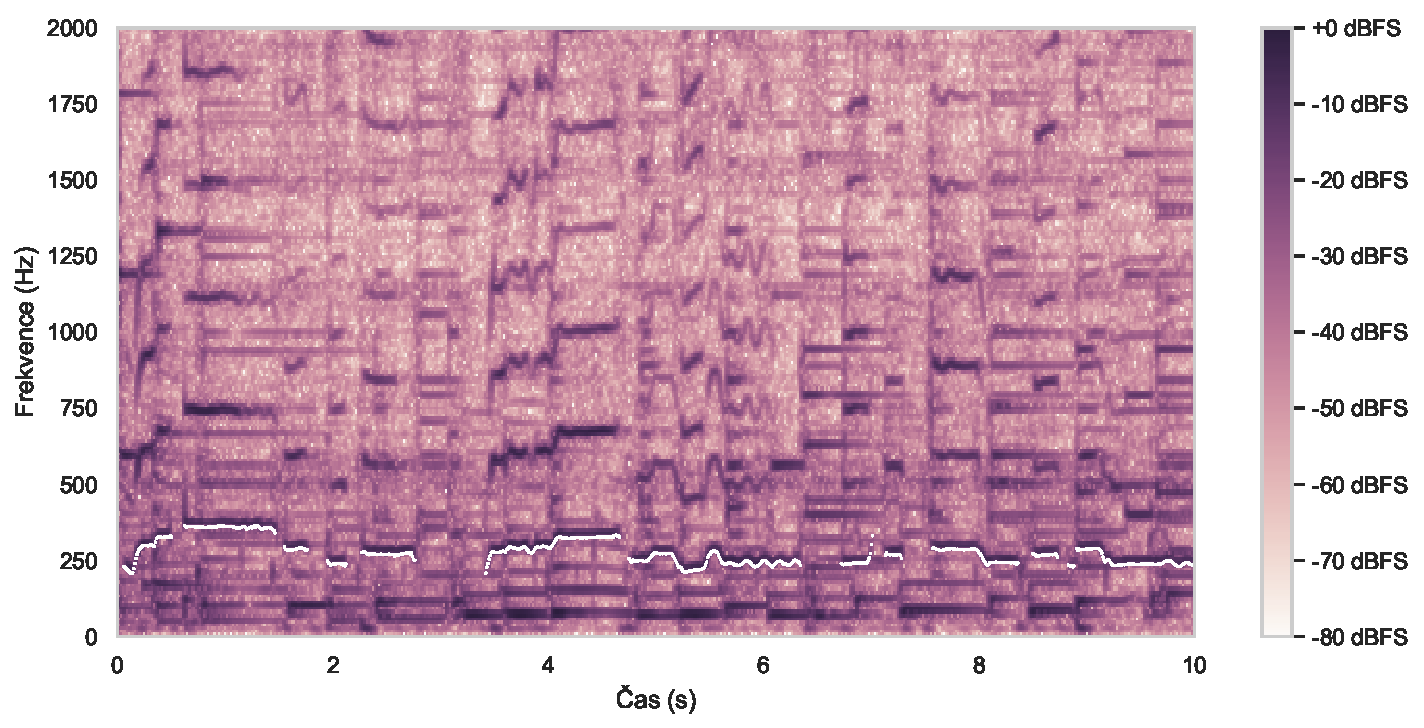
\includegraphics[width=\textwidth,height=\textheight,keepaspectratio]{../img/audio_mix_stft}
\caption{lorem ipsum}
\label{obr:audio_mix_stft}
\end{figure}

Nyní, po objevení harmonické struktury zvuků, jimž lze přiřknout výšku, můžeme přejít k jejich hledání v hudební nahrávce. Obrázek \ref{obr:audio_mix_stft} vznikl pomocí opakované Fourierovy transformace, která byla aplikována na po sobě jdoucí, krátké časové úseky vstupní nahrávky, přičemž intenzity frekvenčních složek v každém časovém okamžiku zvuku jsou nyní znázorněny odstínem barvy. Časově-frekvenční reprezentaci signálu nazýváme obecně \emph{spektrogram}, a jeho výpočet je prvním krokem většiny metod pro extrakci melodie.

- vybudovat intuici o spektrogramu - ukázat bubny
- harmonická povaha intervalů! - ukázat překryv melodie a doprovodu

% Pro $h(n, t)$ funkci vah měnících se v čase, lze signál tónu definovat jako:

%	$$ X_{f_0}(t) = \sum_{n=1}^\infty h(n, t) \cdot \sin(n \cdot f_0 \cdot (2\pi t)) $$



% \begin{figure}[h]\centering
% 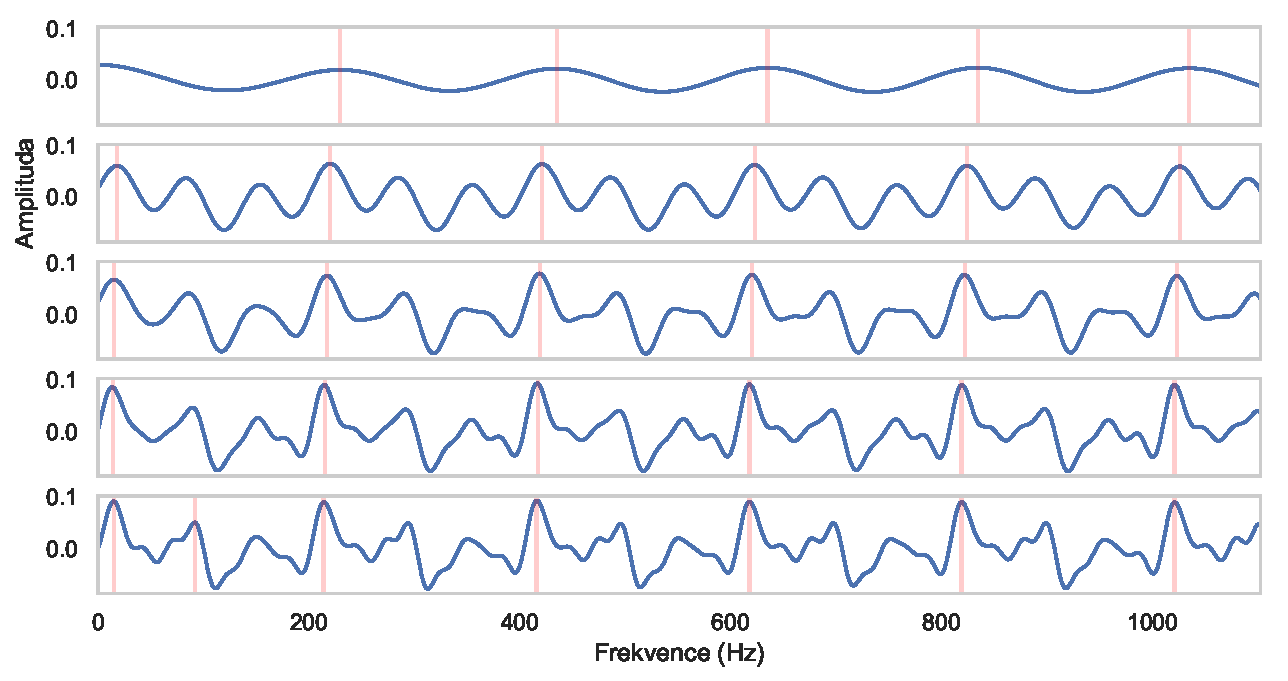
\includegraphics[width=\textwidth,height=\textheight,keepaspectratio]{../img/audio_clarinet_dft_mix}
% \caption{Zvuk klarinetu, postupně vznikající přimícháváním dalších sinusoid}
% \label{obr:audio_clarinet_dft_mix}
% \end{figure}


% tedy rozlišuje jestli se dané vlnění vzduchu opakuje v čase. První z uvedených příkladů zvuků, tedy ty, kterým se dá připsat výška tónu, spojuje právě tato 

% U prvních příkladů  lze snadno představit \uv{vyšší} a \uv{nižší} příklady toho samého zvuku

% Dva zásadní problémy
% - dva zásadní problémy, jako kdyby představovaly osy spektrogramu
% 	- překryv
% 	- definice

\section{Definice melodie}

Rozpoznání melodie hrající skladby je pro většinu posluchačů intuitivní schopností, která je součástí prožitku poslechu hudby, a která jejímu poslechu vůbec dává smysl. Slyšet hudbu a nevnímat melodii je podobné jako poslouchat řeč a nerozumět větám. Ačkoli je melodie tedy termín, který je subjektivně jasný, formální, obecně přijímanou muzikologickou definici, která by se zpětně neodkazovala k posluchači, nemá. 

Z tohoto důvodu si výzkumné týmy zabývající se automatickou transkripcí melodie volí pragmaticky spíše užší definice melodie, se kterými se v jejich kontextu lépe pracuje. Práce \cite{Goto1999}, která je považována za jednu z prvních a důležitých prací v oboru, chápe melodii jako konturu fundamentální frekvence sestávající se z nejsilnějších tónů hrajících v omezeném frekvenčním rozsahu. Tato definice je poměrně úzká, tóny melodie se totiž jistě mohou vyskytovat i mimo autory specifikovaný rozsah a nemusí být vždy v poměru s doprovodem nejsilnější složkou signálu. Z technického hlediska však umožnila autorům implementaci algoritmu běžícího v reálném čase, který poskytoval sémanticky bohatý popis vstupních nahrávek. Navazující články pracují s volnějšími definicemi, které lépe reflektují podstatu melodie. Mimo to se používaná definice proměňuje díky novým datasetům, jejichž autoři tvoří protipól k ryze technickým a objektivním cílům algoritmických metod. Zatímco pro tvorbu algoritmů je praktické zvolit co nejkonkrétnější cíl, při tvorbě datasetu se naopak projevuje lidská subjektivita autorů anotací. 

Kompromisem mezi subjektivní a praktickou definicí se na dlouhou dobu stala \uv{extrakce základní frekvence hlavního melodického hlasu}. Ačkoli melodii v reálném hudebním materiálu obvykle nese více hlasů, které se v hraní střídají (například píseň se zpěvem a kytarovým sólem), v letech 2005 -- 2015 se v soutěži MIREX provádí evaluace pouze nad krátkými výňatky, kde tato definice není omezující. Tento pohled však otevírá také jiné přístupy, například extrakci melodie pomocí modelování hudebního záznamu jako součtu signálu jednoho hlasu a doprovodu \citep{Durrieu2010}, \citep{Bosch2016b} nebo přímo omezení se na separaci lidského zpěvu a doprovodu \citep{Ikemiya2016}. Nově se objevují práce, které \uv{hlavní} melodický hlas neinterpretují nutně jako \uv{nejsilnější}. Skladatelé a hráči používají množství různých postupů, které melodii zvýrazňují --- krom dynamiky ji ovlivňuje například také barva hlasu, vibrato nebo délka not. \cite{Salamon2012a} využívá těchto rysů pro výběr mezi kandidáty na melodickou konturu.

Posunem v rámci MIR komunity bylo zveřejnění nových datasetů MedleyDB \citep{Bittner2014} a ORCHSET \citep{Bosch2016}, oba přináší nová data, ve kterých již melodii nenese pouze jeden hlas po celou dobu skladby. V porovnání s do té doby dostupnými daty jde o mnohem rozmanitější kolekce. V případě MedleyDB jde o první volně dostupný dataset, ve kterém se objevují celé skladby, nikoli pouze výňatky a autoři předkládají rovnou tři verze anotací:

\begin{enumerate}
    \item Základní frekvence nejvýraznějšího melodického hlasu, jehož zdroj zůstává po dobu nahrávky neměnný.
    \item Základní frekvence nejvýraznějšího melodického hlasu, jehož zdroje se mohou měnit.
    \item Základní frekvence všech melodických hlasů, potenciálně pocházejících z více zdrojů.
\end{enumerate}

První formulace je v souladu s doposud používanou definicí. Zbylé dvě se snaží posouvat možné cíle budoucích metod a předložit komunitě nové výzvy, podle \cite{Salamon2014} totiž výzkum začal v letech 2009--2012 stagnovat. Zatímco anotace s jednou melodickou linkou (1. a 2. definice) se v navazujících pracích často používají, zatím žádný článek se nepokusil představit metodu, jejímž cílem by bylo extrahovat více melodických linek (3. definice).

\cite{Bosch2016} při práci na datasetu ORCHSET vychází z článku \cite{Poliner2007}, který definuje melodii jako \uv{jednohlasou sekvenci tónů, kterou bude posluchač nejspíše reprodukovat, pokud jej požádáme o zapískání či zabroukání příslušné skladby}. Přestože nejde o objektivní definici, v praxi se posluchači často na jedné konkrétní sekvenci tónů shodnou, a to jak u populární hudby, kde melodii často nese lidský zpěv, tak u orchestrálních skladeb. Ačkoli se definice neujala pro metody extrakce, \cite{Bosch2016} ji využili pro anotaci výňatků z orchestrálních skladeb, u kterých by předchozí zmíněné definice selhávaly, jelikož pojem melodie je u orchestrální hudby mnohdy komplikovanější než u jiných žánrů. Anotace tak spočívala v přezpívání orchestrálních výňatků skupinou posluchačů a následném srovnání a zpracování těchto nahrávek.

\section{Hluboké učení}

Motivací pro použití metod strojového učení je překonání limitů člověkem navržených, rigidních, pravidlových systémů. Cílem je automatické nalezení optimálního postupu pro řešení úlohy, na základě množství dat, ve kterých strojové učení dokáže nalézt a využít jejich pravidelnosti. V našem případě pak po metodě založené na strojovém učení požadujeme, aby na základě příkladů z trénovací množiny vytvořila funkci salience. 

Výhodou tohoto přístupu je, že o vstupních datech nemusíme dělat žádné předpoklady. Vzniklá metoda pak může v praxi zohledňovat více faktorů ovlivňujících přítomnost melodie, jako je její barva, frekvenční modulace (vibrato, glissando) nebo hlubší vzájemné srovnání současně znějících tónů. Na základě trénovacích příkladů může být tato metoda robustnější vůči většímu spektru barev hlasů nástrojů --- zatímco předešlé metody pro extrakci melodie často uvažují signály s postupně se snižujícím podílem harmonických frekvencí, opravdové signály hudebních nástrojů často tento předpoklad nesplňují (viz obrázek \ref{obr:audio_clarinet_dft}).

První pokus o využití těchto metod představili \cite{Poliner}, vstupní signál transformovali pomocí krátkodobé Fourierovy transformace a část spektra po jednoduché normalizaci použili jako vstupní data pro metodu podpůrných vektorů (SVM). Jejich metoda měla své limitace, výstup byl kvantizován na úroveň jednoho půltónu a tudíž metoda nedokázala dobře postihnout například vibrata. I přesto však tým dosáhl srovnatelných výsledků s tehdejším state-of-the-art. 

Po roce 2005 jakékoli pokusy o aplikaci strojového učení ustávají a na nové metody se čeká až do roku 2016, jedním z důvodů byl jistě nedostatek dat, tuto situaci zlepšil například dataset MedleyDB \citep{Bittner2014} nebo dnes již zaniklý iKala \citep{Chan2015}. Zájem o strojové učení však znovu stoupá s úspěšným využitím hlubokých neuronových sítí napříč obory a tak se na konferenci ISMIR 2016 objevují dva články týmů \cite{Kum2016} a \cite{Rigaud2016}, založené právě na hlubokém učení. V roce 2017 publikuje své metody \cite{Bittner2017} (ISMIR 2017), \cite{Balke2017} (ICASSP 2017), následující rok přináší metody \cite{DBasaranSEssid2018} (ISMIR 2018), \cite{Bittner2018}. V oboru lze tedy od roku 2016 vidět velmi výrazný trend právě směrem k hlubokému učení, a stejný směr je patrný i v příbuzných úlohách přepisu hudby. Tým z laboratoře Google Brain dokázal výrazně zlepšit přepis klavírních skladeb pomocí kombinace konvoluční a rekurentní architektury \citep{Hawthorne2018}. Neuronové sítě také zlepšují výsledky na poli oddělení signálů \citep{Stoller2018}.


% \cite{Thickstun2016} - musicnet
% \cite{Hawthorne2018} - google magenta

% V oboru transkripce hudby se trend v použití hlubokých sítí